\documentclass[tikz,border=8pt]{standalone}
% Shared look for every TikZ diagram. Load with \input{../../tools/tikz-style.tex}
\usepackage[T1]{fontenc}
\usepackage{lmodern}
\renewcommand{\sfdefault}{lmr}  % diagrams use the same serif as the text
\usetikzlibrary{arrows.meta, positioning, shapes.geometric, calc, fit, backgrounds}
\definecolor{cblue}{HTML}{4C78A8}
\definecolor{corange}{HTML}{F58518}
\definecolor{cgreen}{HTML}{54A24B}
\definecolor{cred}{HTML}{E45756}
\definecolor{cpurple}{HTML}{B279A2}
\definecolor{cgrey}{HTML}{6B6B6B}
\tikzset{
  every picture/.style={font=\sffamily, line width=1.2pt},
  box/.style={draw=#1, fill=#1!12, rounded corners=4pt, align=center, inner sep=7pt, minimum height=1.1cm},
  box/.default=cgrey,
  arrow/.style={-{Stealth[length=3mm]}, draw=cgrey, line width=1.4pt},
  title/.style={font=\sffamily\bfseries\Large},
  note/.style={font=\sffamily\small, text=cgrey, align=center},
}
\AtBeginDocument{\hyphenpenalty=10000 \exhyphenpenalty=10000}

% Left: holonomic. A train on a circular track x^2 + y^2 = 25 can only be on the circle; at (3, 4) its velocity is along the track.
% Right: nonholonomic. At one pose the robot can only move along its heading (green) or turn, never sideways (red), yet it can reach any pose.
\begin{document}
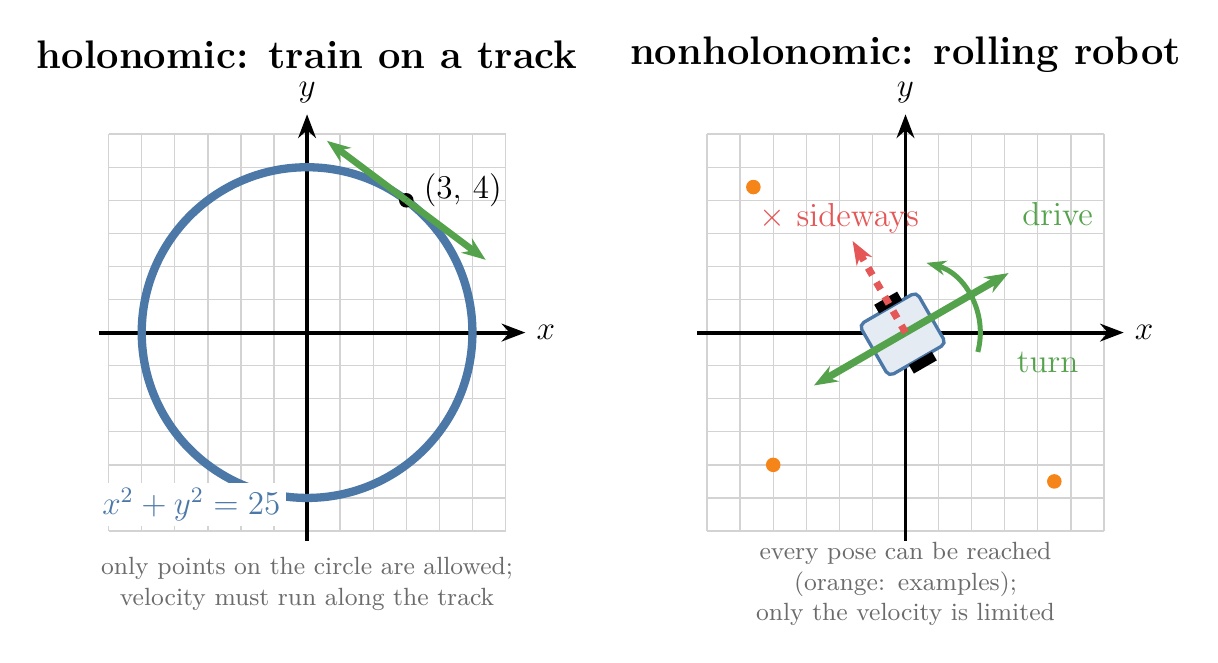
\begin{tikzpicture}[every node/.append style={font=\large}]
  \begin{scope}[scale=0.42]
    \node[title] at (0,8.4) {holonomic: train on a track};
    \draw[cgrey!30, line width=0.5pt] (-6,-6) grid (6,6);
    \draw[arrow, draw=black] (-6.3,0) -- (6.6,0) node[right] {$x$};
    \draw[arrow, draw=black] (0,-6.3) -- (0,6.6) node[above] {$y$};
    \draw[cblue, line width=3pt] (0,0) circle (5);
    \node[cblue, fill=white, inner sep=2pt] at (-3.5,-5.2) {$x^2 + y^2 = 25$};
    \fill[black] (3,4) circle (0.22);
    \node[right] at (3.2,4.3) {$(3,\,4)$};
    \draw[-{Stealth[length=3mm]}, cgreen, line width=2.4pt] (3,4) -- (0.6,5.8);
    \draw[-{Stealth[length=3mm]}, cgreen, line width=2.4pt] (3,4) -- (5.4,2.2);
    \node[note, text width=6.5cm] at (0,-7.6) {only points on the circle are allowed;\\velocity must run along the track};
  \end{scope}
  \begin{scope}[xshift=7.6cm, scale=0.42]
    \node[title] at (0,8.4) {nonholonomic: rolling robot};
    \draw[cgrey!30, line width=0.5pt] (-6,-6) grid (6,6);
    \draw[arrow, draw=black] (-6.3,0) -- (6.6,0) node[right] {$x$};
    \draw[arrow, draw=black] (0,-6.3) -- (0,6.6) node[above] {$y$};
    \begin{scope}[rotate=30]
      \draw[cblue, fill=cblue!15, rounded corners=2pt] (-1.1,-0.9) rectangle (0.9,0.9);
      \fill[black] (-0.4,0.9) rectangle (0.4,1.2);
      \fill[black] (-0.4,-1.2) rectangle (0.4,-0.9);
      \draw[-{Stealth[length=3mm]}, cgreen, line width=2.6pt] (0,0) -- (3.6,0);
      \draw[-{Stealth[length=3mm]}, cgreen, line width=2.6pt] (0,0) -- (-3.2,0);
      \draw[-{Stealth[length=3mm]}, cred, line width=2.6pt, dashed] (0,0) -- (0,3.2);
      \node[cred] at (0,4.0) {$\times$ sideways};
      \draw[-{Stealth[length=2.5mm]}, cgreen, line width=1.8pt] (1.6,-1.6) arc (-45:45:2.2);
    \end{scope}
    \node[cgreen] at (4.6,3.6) {drive};
    \node[cgreen] at (4.3,-0.9) {turn};
    \fill[corange] (-4,-4) circle (0.22); \fill[corange] (4.5,-4.5) circle (0.22); \fill[corange] (-4.6,4.4) circle (0.22);
    \node[note, text width=6.5cm] at (0,-7.6) {every pose can be reached (orange: examples);\\only the velocity is limited};
  \end{scope}
\end{tikzpicture}
\end{document}
